%%%%%%%%%%%%%%%%%%%%%%%%%%%%%%%%%%%%%%%%%%%%%%%%%%%%%%%%%%%%%%%%%%%%%%%%%%%%%%%%%%%%%%%%%%%
%                               Evaluation - 16pp
%%%%%%%%%%%%%%%%%%%%%%%%%%%%%%%%%%%%%%%%%%%%%%%%%%%%%%%%%%%%%%%%%%%%%%%%%%%%%%%%%%%%%%%%%%%
\chapter{Evaluation}
\label{sec:evaluation}

\section*{Summary}
%To evaluate our approach we plan to run several experimental tests within a group of, at least, ten subjects. 
%With these experiments we want to obtain statistical measures about our approach and be able to conclude 
%on which combinations of feedback could have better performance in guiding a patient.

%We will be using two different experiments in order to achieve comparable results. 
%The first experiment will consist of a \ac{PT} and a test subject. 
%The \ac{PT} will demonstrate a given exercise to the test subject and then evaluate their execution without giving any kind of feedback. 

%The second experiment will involve guiding a test subject through the same exercise as the first experiment, 
%using different combinations of visual, audio and haptic feedback.
%The resulting performance will be analyzed and several data gathered. 
%We will take into account the following metrics, (a) the trajectory error between the Exercise Model and 
%the patient's actual execution, (b) the time it takes for the patient to finish the exercise 
%and (c) the time it takes for the patient to recover to the correct position if mistaken.

%We will start by using a unimodal approach, to obtain measurements using only one of the 
%available feedback modes each time. After the unimodal experiments, we will begin the multimodal 
%approach experiments by combining the available feedback and repeat the same measurements previously done.

%Even though our main focus is to provide concurrent feedback (during the execution), its frequency will be altered in order to evaluate the patient response. Therefore, further in the end, we will provide only terminal feedback (without guiding cues during the execution) to analyze if the patient successfully learned the movement.

For the evaluation of the SleeveAR, we intended to observe how well could a subject recreate simple arm movements by only following the feedback at his disposal. In this section we will present a detailed description of the type of tests that were made, what type of information was being gathered and also highlight some of the most important critics received by a professional physical therapist after using our system.

Since the test would involve executing simple arm movements, five different exercises were created for this evaluation. \todo{colocar links de youtube?} These exercises were recorded both by video and by the SleeveAR's Learning Architecture at the same time. This way, we knew for certain that it was the same movement being stored in video and in our system.

In this chapter we present the methodology used for testing our prototype with test subjects. All the results will be discussed in order to achieve a better understanding about our prototype success. In the end a meeting with a physical therapist, from which resulted a great discussion and exchange of ideas, will also be fully reported.

\section{Methodology} \label{evaluation-methodology}

\begin{table}
\centering
\begin{tabular}{lll}
\hline
\multicolumn{1}{|l|}{\#}& \multicolumn{1}{l|}{Stage}         & \multicolumn{1}{l|}{Time}       \\ \hline
\multicolumn{1}{|l|}{1} & \multicolumn{1}{l|}{Introduction}  & \multicolumn{1}{l|}{2 minutes}  \\ \hline
\multicolumn{1}{|l|}{2} & \multicolumn{1}{l|}{SleeveAr}      & \multicolumn{1}{l|}{15 minutes} \\ \hline
\multicolumn{1}{|l|}{3} & \multicolumn{1}{l|}{Video}         & \multicolumn{1}{l|}{10 minutes} \\ \hline
\multicolumn{1}{|l|}{4} & \multicolumn{1}{l|}{Questionnaire} & \multicolumn{1}{l|}{3 minutes}  \\ \hline
\end{tabular}
\caption{SleeveAR evaluation stages}
\label{table:teststages}
\end{table}

%\begin{itemize}
%\item divided by 3 main parts
%\item executing movements following video instructions
%\item executing movements following SleeveAR
%\item answering a small form at the end
%\end{itemize}

In this section we describe what methodologies were used to test our prototype. Each of our participants followed this methods similarly.

The average time spent with each participant was approximately thirty minutes. The test was composed of four stages as we can observe in Table \ref{table:teststages}.

\begin{enumerate}
\item \textbf{Introduction}

Before the actual test, a brief explanation was given about the main goal of our thesis. The participants were also made aware of what would the full experimental test consist of.

\item \textbf{SleeveAR}

The participant would have to execute exercises, described in section \ref{evaluation-tasks}, while following our prototype real-time feedback.

\item \textbf{Video}

For each of the five exercises selected for this evaluation, the participant would have to watch a video of its execution at least two times. Then, while following the video playing, the participant would execute the same movement based on what he was observing.

\item \textbf{Questionnaire}

Finally, a small questionnaire would be filled by the participant. This questionnaire included questions about stage 2 and 3 while also providing us some information about the user's profile.

\end{enumerate}

In order to gather data for further result analysis, each execution of an exercise generated a Log with all the necessary information about the participant's movement. \todo{descrever Logs mais detalhadamente}

Even though we are ordering the stages this way, half of the participantes started by doing the third stage before the second, for the purpose of obtaining a more balanced sample of results.

\section{Performed Tasks} \label{evaluation-tasks}
For both the second and third stage described in the previous section, the same five exercises were executed.

Each exercise was simultaneously recorded witg a video camera and with motion tracking devices. Under these circunstances, we made sure that the content being stored in video format directly represented the data being stored on SleeveAR's architecture.
The tasks performed in stage 2 and 3 had the same goal of recreating the five exercises recorded.

\todo{explicar como era cada exercicio?}

\section{Environment and Participants} 



\section{Results}

The empirical evaluation addressed the correctness of the executed exercises. Experiments with test subjects were performed for a baseline scenario, consisting of exercise execution through video observation, and for the proposed prototype. The performance metrics is given by the degree of similarity between the participants' arm trajectories and the original trajectories demonstrated by the therapist. It is measured using the \textbf{\ac{DTW}} \todo{referencia para o algoritmo} algorithm, 
which is appropriate for measuring a degree of similarity between two temporal sequences which may vary in time or speed. With the application of this algorithm in mind, the recorded movements can be reformulated as a sequence of positions. One can then compare the performance values for both the proposed solution and the baseline scenario.

Due to an arm movement being divided by the upper and fore arm sections, the \ac{DTW} was applied to each individually, thus providing us with a more detailed set of values. By doing said division, we could observe if there were notable performance differences between each arm region.

The final \ac{DTW} values of each exercise are the result of adding both arm regions' DTW values. It is important to highlight that with the following results, DTW values closer to zero directly represent movements more similar to the original.

For the first exercise, we can observe in Figure \ref{fig:sleevearVSvideoEx1} the test results from all participants, both using the SleeveAr and by observing the respective video.

These results clearly show SleeveAR provided a higher similarity when comparing to the original exercise. In terms of statistic values, participantes achieved an average \ac{DTW} value of \textbf{0.114181315} and a Standard Deviation of \textbf{0.090349091} when using SleeveAR, as oppose to an average \ac{DTW} value of \textbf{0.438959688} and a standard deviation of \textbf{0.164684962}

\begin{figure}[t!]
    \centering
    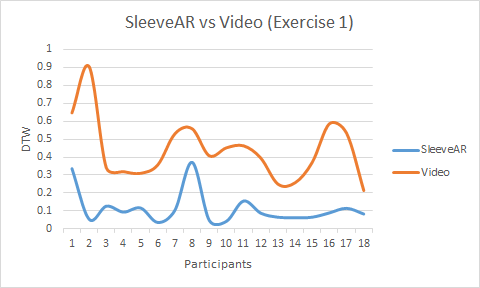
\includegraphics{imgs/results/sleevearVSvideoEx1.png}
    \caption{Exercise 1 DTW comparison between SleeveAR and observing video.}
    \label{fig:sleevearVSvideoEx1}
\end{figure}

\section{Validation with Physical Therapist}

We had the opportunity of meeting with a professional physical therapist which accepted our invitation to test the SleeveAR prototype and provide us with some feedback in a small interview.

Prior to the interview, it as decided that the therapist would be part of the same tests being done for our evaluation, which have already been described in this chapter \todo{ref}. Under those circumstances we were able to demonstrate the full potential of our prototype and, as a result of these tests, we received some very interesting feedback.

First of all, this prototype main vision was to prove we were able to guide subjects through pre-recorded exercises in order for them to be as close as possible of the original exercise. With this in mind, we wanted to know in what way would this kind of tool be useful in a regular physical therapy work environment. We also wanted to understand what would be missing to make SleeveAR a more complete tool for a common use along this field of rehabilitation.

We will now present the most notable feedback received, both positive and negative.




\begin{itemize}
\item \textbf{Missing feedback from one of the three axis}

For SleeveAR feedback to be fully complete, it would need to take into account the missing axis of movement in its real-time feedback. Since this prototype focused on guiding the arm through relatively simple movements, we did not detect this problem. But, consequently, in the evaluation tests, we realized that it might have helped to take this into account. In Fig \textbf{fazer figura} we can see an example where, without verifying the upper arm's rotation, our system considers both arm poses to be the same. This happens because both the upper arm direction and angle between the upper and fore arm remain the same.


\item \textbf{Arm obstructs visibility}

Ocasionally, the right arm might obstruct the user's vision, making it difficult to observe the feedback being projected onto the floor. This issue could be solved by projecting all the visual feedback further away from the subject

\item \textbf{Increase number of tracking points in shoulder area}

In physical therapy, a lot of arm movements also focus on the shoulder area. With this in mind, it would be necessary for our sleeve to contain more tracking points around the shoulder instead of only having a tracking point for the shoulder, elbow and wrist.

\item \textbf{Potential useful tool for patient reports}

Some physical therapists follow a group of standard arm movements to initially evaluate a patient's condition. With this tool, they could receive full reports with necessary data that otherwise they would have to measure physically. It could be possible to extend SleeveAR to return several additional information about a patient's range of movement after executing a group of exercises. This would allow a physical therapist to have access to information much faster and, possibly, more precise about the patient. 

Also, with the possibility of recording movements and later replaying them, SleeveAR could offer a great way of demonstrating the patient, in a visual form, how much he has improved over the course of his rehabilitation, by replaying the recordings of his movements.

\item \textbf{A great tool to help a physical therapist when multi-tasking}

While working in a physical therapy gymnasium, therapists often have to look after several patients at the same time. Tools like SleeveAR could help the therapist by lowering the amount of times they have to correct a patient and, therefore, focus on another patient that might need more priority help.


\item \textbf{Provides a great motivation with the feedback received}

The \ac{KP} and \ac{KR} demonstrated in SleeveAR is very satisfactory and could really help in motivating a patient while showing his evolution as he keeps repeating the exercises.

Being able to show how the patient performed by drawing his trajectory over the original exercises helps understanding which parts need improvement. Also, the real-time feedback does a great job at instantaneously showing the patient what to correct on his exercise.

\end{itemize}

\section{Discussion}

results x therapist 